%%%%%%%%%%%%%%%%%%%%%%%%%%%%%%%%%%%%%%%%%%%%%%%%%%%%%%%%%%%%%%%%%%%%%%%%%%%%%%%%
%                    Capitulo 2: Antecedentes                                  %
%%%%%%%%%%%%%%%%%%%%%%%%%%%%%%%%%%%%%%%%%%%%%%%%%%%%%%%%%%%%%%%%%%%%%%%%%%%%%%%%

\chapter{Antecedentes}

\section{Trabajos relacionados}

Hasta donde sabemos, no se ha desarrollado una arquitectura de planificación para
controlar el comportamiento deliberativo de un agente en \texttt{GVGAI}. No
obstante, se han desarrollado otras arquitecturas de planificación para otros juegos,
como es el caso de StarCraft. Algunas de estas arquitecturas son, por ejemplo,
\texttt{Darmok} \cite{10.1007/978-3-540-74141-1_12}, basada en casos;
\texttt{UalbertBot} \cite{Churchill2011BuildOO}, basada en la búsqueda heurística de
planes concurrentes; \texttt{EISBot} \cite{Weber2011BuildingHA}, basada en planificación reactiva;
y una arquitectura basada en \texttt{PELEA} \cite{Alczar2010peleaP} que combina
\textit{goal reasoning} \cite{Aha_2018} con planificación clásica.

A diferencia de las anteriores, nuestra arquitectura está diseñada para resolver
problemas en varios dominios de planificación y juegos en vez de solo en un
dominio de planificación y un juego, que en este caso sería StarCraft.
Por esa razón, presentamos una metodología semiautomática para la integración de un
planificador en cualquier juego de \texttt{GVGAI} que pueda ser resuelto mediante
planificación.

\section{Planificación automática}

La planificación automática es un área de la IA que se encarga del estudio de
técnicas que permiten resolver problemas en los que, dado un objetivo determinado,
se debe buscar una serie de acciones que permitan alcanzarlo \cite{10.5555/3073924}.

Para resolver problemas de planificación se requieren tres elementos:

\begin{itemize}[label=\textbullet]
    \item Un \textbf{dominio de planificación}, el cual representa un entorno y las acciones
    que puede realizar un actuador en ese entorno, además de cómo dichas acciones afectan
    al entorno.
    \item Un \textbf{problema de planificación}, en el cual representa un estado inicial
    concreto de un entorno y un objetivo que debe ser alcanzado por el actuador.
    \item Un \textbf{planificador}, que es un programa que recibe como entradas un dominio y un
    problema de planificación y devuelve un conjunto de acciones ordenadas que debe realizar
    el agente para alcanzar el objetivo desde el estado inicial descrito en el problema de
    planificación.
\end{itemize}

La planificación ha supuesto un gran impacto en la IA, ya que ha permitido el desarrollo
de agentes cuya componente deliberativa se basa en dichas técnicas. Estos agentes, normalmente,
siguen una arquitectura basada en \textbf{planificación}, \textbf{percepción} y \textbf{ejecución}:

\begin{itemize}
    \item La componente de \textbf{planificación} ya es conocida. Permite obtener una serie
    de accione que permiten al agente alcanzar un objetivo determinado.
    \item La componente de \textbf{percepción} permite al agente obtener información sobre
    su entorno, utilizando para ello sensores. Estos sensores pueden ser reales (por ejemplo
    una cámara) o simulados (por ejemplo, en un videojuego se puede simular lo que
    ve un agente, simulando así una cámara).
    \item La componente de \textbf{ejecución} permite ejecutar el plan y controlar su ejecución
    en todo momento, de forma que se puede saber por ejemplo cuando detener la ejecución. Normalmente
    de esto último se encarga un módulo de \textbf{monitorización}, el cual está incluido en la componente
    de ejecución.
\end{itemize}

A pesar de que la planificación ha sido integrada con éxito en ciertas áreas, como por ejemplo la robótica,
los vehículos no tripulados o los sistemas de producción, hay un área en el cual su integración es más
complicada: los videojuegos. El motivo de esto se debe a que la mayoría de videojuegos presentan
entornos dinámicos en cambio continuo y/o con un número extremadamente alto de acciones entre las que escoger.
Planificar suele ser un proceso costoso, ya que los espacios de búsqueda suelen ser bastante grandes y por tanto,
suelen ofrecer una respuesta relativamente lenta. Al estar estos entornos en cambio continuo,
un plan que se haya obtenido deja de ser válido al cabo de poco tiempo, lo cual implica estar
replanificando constantemente. En un estudio realizado \cite{10.1111/coin.12079} se ha visto que en entornos
de este tipo (muy dinámicos) o muy grandes, un agente reactivo es capaz de ofrecer una respuesta similar
a la que permite obtener una arquitectura basada en planificación solo que en un tiempo muchísimo menor. 

\subsection{\texttt{PDDL}}

\texttt{PDDL} (\textit{Planning Domain Definition Language}) \cite{pddl} es uno de los lenguajes más utilizados
para la representación de dominios y problemas de planificación. Surgió a finales de los 90
como un intento de estandarizar los lenguajes que se utilizan para describir los dominios
y problemas de planificación. Desde su aparición, el lenguaje ha experimentado una serie de cambios que
han añadido funcionalidad nueva al lenguaje. Además, a partir de él han surgido otros lenguajes de planificación.

Un dominio de planificación de \texttt{PDDL} puede contener los siguientes elementos:

\begin{itemize}[label=\textbullet]
    \item Un nombre de dominio. Este elemento es obligatorio
    \item Unos requisitos del dominio, denotados por \texttt{:requirements}.
    \item Uno o varios tipos, que representan de forma general los elementos que aparecen
    en el entorno. Se denotan por \texttt{:types}, y su uso, aunque no es obligatorio, simplifica
    mucho la legibilidad del dominio.
    \item Una serie de predicados, los cuales expresan características de los elementos
    y del entorno. Se denotan mediante \texttt{:predicates}. Su uso es obligatorio.
    \item Funciones, las cuales son predicados que almacenan un valor numérico. Se denotan
    mediante \texttt{:functions} y su uso no es obligatorio.
    \item Acciones, las cuales representan la manera en la que el agente interactúa con
    el entorno y los elementos de éste. Se denotan utilizando \texttt{:action}.
    
    Una acción se compone de unos \textbf{parámetros} (representados por \texttt{:parameters}), que son
    una serie de instancias concretas u objetos; unas \textbf{precondiciones} (\texttt{:precondition}),
    que son una serie de predicados que se tienen que cumplir en el estado actual del problema cuando
    se sustituyen las variables de dichos predicados por las instancias concretas recibidas como parámetro;
    y una lista de \textbf{efectos} (\texttt{:effect}), la cual indica como cambia el entorno cuando
    el agente realiza dicha acción.
\end{itemize}

Por otro lado, un problema de planificación de \texttt{PDDL} se compone de los siguientes elementos:

\begin{itemize}[label=\textbullet]
    \item Un nombre de problema.
    \item El dominio \texttt{PDDL} que se utiliza en el problema, denotado por \texttt{:domain}.
    \item Una lista de instancias que componen el estado del problema, denotada por \texttt{:objects}.
    \item Una lista con los predicados instanciados que indican el estado inicial
    del problema. Esta lista se denota mediante \texttt{:init}.
    \item Una serie de objetivos que se deben alcanzar, denotados por \texttt{:goal}.
\end{itemize}

Para entenderlo mejor, vamos a ver un pequeño ejemplo. Supongamos que queremos representar un
dominio en el que hay dos tipos de elementos: monedas y frascos. Una persona puede coger una moneda,
la cual se encuentra en el suelo, y puede ponerla en un frasco. Solo se puede coger una moneda a la vez.
Además, se quiere llevar la cuenta de cuántas monedas hay en un frasco.

El dominio \texttt{PDDL} que representaría dicha descripción sería el siguiente:

\begin{lstlisting}[language=PDDL,caption={Ejemplo de dominio \texttt{PDDL}.},captionpos=b]
(define (domain COINS)
  (:requirements :strips :typing :fluents)
  (:types
    Coin Jar
  )
  (:predicates
    (in ?c - Coin ?j - Jar)
    (on-floor ?c - Coin)
    (taken ?c - Coin)
    (empty-hand)
  )
  (:functions
    (coins-in-jar ?j)
  )
  (:action pick
     :parameters (?c - Coin)
     :precondition (and
       (empty-hand)
       (on-floor ?c)
     )
     :effect (and
       (not (empty-hand))
       (not (on-floor ?c))
       (taken ?c)
     )
  )
  (:action store
     :parameters (?c - Coin ?j - Jar)
     :precondition (taken ?c)
     :effect (and
       (not (taken ?c))
       (in ?c ?j)
       (empty-hand)
       (increase (coins-in-jar ?j) 1)
     )
  )
)
\end{lstlisting}

Ahora, vamos a suponer que queremos representar un problema en el que hay tres monedas
(\texttt{c1}, \texttt{c2} y \texttt{c3}) y un frasco (\texttt{j1}). Las tres monedas están en
el suelo y no hay ninguna en el frasco. Queremos conseguir que en el frasco haya dos monedas y que una
de ellas, \texttt{c1}, esté dentro del frasco. El problema \texttt{PDDL} que representaría la descripción
anterior es el siguiente:

\begin{lstlisting}[language=PDDL,caption={Ejemplo de problema \texttt{PDDL}.},captionpos=b]
(define (problem CoinProblem)
  (:domain COINS)
  (:objects
    c1 c2 c3 - Coin
    j1 - Jar
  )
  (:init
    (empty-hand)
    (on-floor c1)
    (on-floor c2)
    (on-floor c3)
    (= (coins-in-jar j1) 0)
  )
  (:goal
    (AND
      (in c1 j1)
      (= (coins-in-jar j1) 2)
    )
  )
)
\end{lstlisting}

Como es de suponer \texttt{PDDL} contiene muchos otros elementos. De entre ellos se quieren destacar los efectos
condicionales. Estos son efectos de una acción que tienen lugar siempre y cuando las condiciones sean satisfechas
en el estado actual del problema. Un ejemplo de esto se puede ver en la siguiente acción, la cual se ha extraído
de un dominio escrito para un juego de \texttt{GVGAI} llamado \textit{Ice and Fire}:

\begin{lstlisting}[language=PDDL, caption={Ejemplo de efecto condicional.},captionpos=b]
  (:action pick-boots
    :parameters (?a - Avatar ?c - Cell ?b - Boots)
    :precondition (and
      (at ?a ?c)
      (at ?b ?c)
    )
    :effect (and
      (when
        (fire-boots ?b)
        (has-fire-boots ?a)
      )
      (when
        (ice-boots ?b)
        (has-ice-boots ?a)
      )
      (not (at ?b ?c))
    )
  )
\end{lstlisting}

El funcionamiento del juego se explicará más detalladamente en capítulos posteriores. De aquí
lo único que hace falta entender es que con esta acción un avatar intenta coger unas botas cuando
ambos están en la misma casilla y, dependiendo del tipo de las botas, se indica que
el avatar posee uno u otro tipo de botas.

\subsection{\texttt{Planning.Domains}}

\texttt{Planning.Domains} \cite{muise-icaps16demo-pd} es una página \textit{web} que contiene
una colección de herramientas que permiten trabajar con planificación. \url{http://planning.domains/}. 

\section{\texttt{GVGAI}}

\texttt{GVGAI} (General Video Game AI) \cite{7038214} es un entorno de juegos que permite
el desarrollo de agentes basados en Inteligencia Artificial General, es decir, agentes que sean
capaces de resolver múltiples juegos en vez de solo uno en concreto. Cuenta con más de 100 juegos,
los cuales están definidos en \texttt{VGDL} y presentan diferentes tipos de retos para un agente.

\begin{figure}[H]
    \centering
    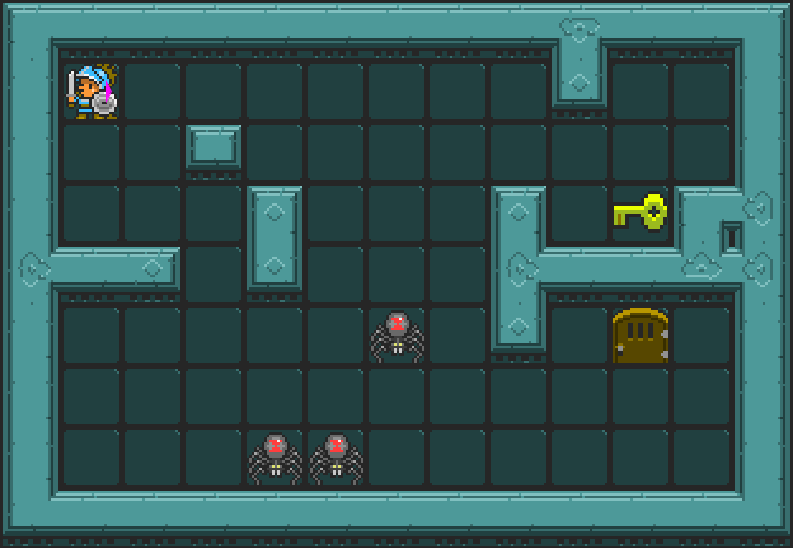
\includegraphics[scale=0.4]{img/CH02/zelda.png}
    \caption{Juego \textit{Zelda} en \texttt{GVGAI}}.
    \label{fig:zelda}
\end{figure}

El entorno está pensado para el desarrollo de agentes reactivos, los cuales se basan por ejemplo en
Aprendizaje por Refuerzo, Algoritmos Genéticos o MCTS (\textit{Monte Carlo Tree Search}). Esto, entre
otras cosas, implica que los tiempos de respuesta de los agentes tienen que ser pequeños. Por tanto,
los agentes deliberativos se encuentran con un problema aquí, ya que suelen tardar más tiempo en ofrecer
una respuesta. Y, como sabemos, los planificadores tardan algún tiempo en dar con una solución. Pero además,
existe otro problema, que es la representación de los juegos y de las acciones del agente en
dominios de planificación. Este proceso puede llegar a ser extremadamente complejo dependiendo
del juego, ya que hay comportamientos que no pueden ser modelados de forma sencilla dentro del juego.
Además, supone cierto esfuerzo crear los dominios y validarlos, ya que hay que entender muy bien las reglas
del juego y las interacciones que pueden suceder. Esto, sin embargo, no significa que integrar una arquitectura
basada en planificación en el entorno sea imposible, pero sí que requiere algo más de trabajo.

\subsection{\texttt{VGDL}}

\texttt{VGDL} (Video Game Description Language) \cite{Schaul2013AVG} es un lenguaje que se
utiliza para la descripción de juegos 2D.

La descripción de un juego consiste de dos componentes:

\begin{itemize}
    \item \textbf{Descripción del nivel}: Se describe la disposición
    de un nivel y la posición de los objetos que están en dicho nivel. Se trata
    de un archivo de texto que compuesto por líneas de la misma longitud, donde
    cada carácter se corresponde con un objeto en una posición que viene dada por la fila
    y la columna en la que se encuentra el carácter.
    \item \textbf{Descripción del juego}: Aquí se describe la dinámica del juego y las
    interacciones entre los distintos objetos que se puedan encontrar en él. Un fichero
    de este tipo contiene los siguientes elementos:
    \begin{itemize}
        \item \texttt{LevelMapping}: Especifica una correspondencia entre los caracteres del archivo
        de descripción del nivel y uno o más objetos que se hayan especificado para cada uno de ellos.
        \item \texttt{SpriteSet}: Especifica los objetos del juego y sus propiedades. Los objetos
        se pueden definir de forma jerárquica mediante la indentación. Los objetos hijo heredan las propiedades
        de su padre y solo pueden tener un único padre.
        \item \texttt{InteractionSet}: Describe las interacciones que tienen lugar cuando dos objetos
        colisionan. El primer objeto causa la interacción y el segundo la recibe.
        \item \texttt{TerminationSet}: Describe las formas en las que puede terminar el juego. Cada
        línea representa un criterio de terminación.
    \end{itemize}
\end{itemize}

\begin{figure}[H]
    \centering
    \begin{subfigure}[b]{.22\textwidth}
    \centering
    \begin{lstlisting}[basicstyle=\small]
wwwwwwwwwwwww
wA.......w..w
w..w........w
w...w...w.+ww
www.w2..wwwww
w.......w.g.w
w.2.........w
w.....2.....w
wwwwwwwwwwwww
    \end{lstlisting}
    \caption{Fichero descripción del nivel.}
    \end{subfigure}%
    \begin{subfigure}[b]{.78\textwidth}
    \centering
    \begin{lstlisting}[basicstyle=\tiny]
BasicGame
  SpriteSet
    floor > Immovable randomtiling=0.9 img=oryx/floor3 hidden=True
    goal  > Door color=GREEN img=oryx/doorclosed1
    key   > Immovable color=ORANGE img=oryx/key2
    sword > OrientedFlicker limit=5 singleton=True img=oryx/slash1
    movable >
      avatar  > ShootAvatar   stype=sword frameRate=8
        nokey   > img=oryx/swordman1
        withkey > color=ORANGE img=oryx/swordmankey1
      enemy >  
        monsterQuick > RandomNPC cooldown=2 cons=6 img=oryx/bat1
        monsterNormal > RandomNPC cooldown=4 cons=8 img=oryx/spider2
        monsterSlow > RandomNPC cooldown=8 cons=12 img=oryx/scorpion1
      wall > Immovable autotiling=true img=oryx/wall3
      	

  LevelMapping
    g > floor goal
    + > floor key        
    A > floor nokey
    1 > floor monsterQuick
    2 > floor monsterNormal
    3 > floor monsterSlow
    w > wall
    . > floor
    

  InteractionSet
    movable wall  > stepBack
    nokey goal    > stepBack
    goal withkey  > killSprite scoreChange=1
    enemy sword > killSprite scoreChange=2
    enemy enemy > stepBack
    avatar enemy > killSprite scoreChange=-1
    nokey key     > transformTo stype=withkey scoreChange=1 killSecond=True

  TerminationSet
    SpriteCounter stype=goal   win=True
    SpriteCounter stype=avatar win=False
    \end{lstlisting}
    \caption{Fichero descripción del juego.}
    \end{subfigure}

    \caption{Descripción en \texttt{VGDL} del juego \textit{Zelda}.}
    \label{fig:vgdl_zelda}
\end{figure}

En la figura \ref{fig:vgdl_zelda} se muestra un ejemplo de un fichero de descripción del nivel
y de descripción del juego para el juego \textit{Zelda}, el cual puede verse en la figura \ref{fig:zelda}.

Los ficheros \texttt{VGDL} de un juego son bastante útiles a la hora de construir un dominio \texttt{PDDL}
para dicho juego, ya que permiten conocer qué objetos hay en ese juego y algunas de las posibles interacciones
entre ellos. Además, estos ficheros son utilizados para generar ficheros de configuración para el sistema, aunque
eso se verá más adelante.
